\documentclass[a4paper, 10pt]{article}

\usepackage{datenumber}
\usepackage{fontsize}
\usepackage{fontawesome5}
\usepackage{fp}
\usepackage{geometry}
\usepackage{graphicx}
\usepackage{hyperref}
\usepackage{multicol}
\usepackage{xcolor}

\geometry{margin=10mm}
\graphicspath{ {../assets/imgs/} }
\pagenumbering{gobble}
\setlength{\tabcolsep}{18pt}
\definecolor{link}{HTML}{56949f}
\definecolor{code}{HTML}{575279}
\hypersetup{
    colorlinks,
    urlcolor=link
}

\newcommand{\link}[2]{\href{#1}{\texttt{#2}}}
\newcommand{\code}[1]{\textcolor{code}{\texttt{#1}}}


\begin{document}

\begin{minipage}[b]{0.68\linewidth}
	{\Huge{\textbf{Harrison Cook}}}
	\vspace{2mm}

	{\Large{Software Engineer}}
	\vspace{5mm}

	\begin{tabular}{|l l|}
		\faIcon{at}             & \link{mailto:contact@honsoncooky.dev}{contact@honsoncooky.dev}                                                                                                                                                                   \\
		\faIcon{edge}           & \link{https://about.honsoncooky.dev}{about.honsoncooky.dev}                                                                                                                                                                      \\
		\faIcon{github}         & \link{https://github.com/honsoncooky}{github.com/honsoncooky}                                                                                                                                                                    \\
		\faIcon{linkedin}       & \link{https://www.linkedin.com/in/honsoncooky}{linkedin.com/honsoncooky}                                                                                                                                                         \\
		\faIcon{map-marker-alt} & \link{https://www.google.co.nz/maps/place/Wellington/@-41.2528426,174.5894495,11z/data=!3m1!4b1!4m6!3m5!1s0x6d38b1fc49e974cb:0xa00ef63a213b470!8m2!3d-41.2923814!4d174.7787463!16zL20vMDg1M2c?entry=ttu}{Wellingon, New Zealand}
	\end{tabular}
\end{minipage}
\hfill
\begin{minipage}{0.28\linewidth}
	\centering
	\fbox{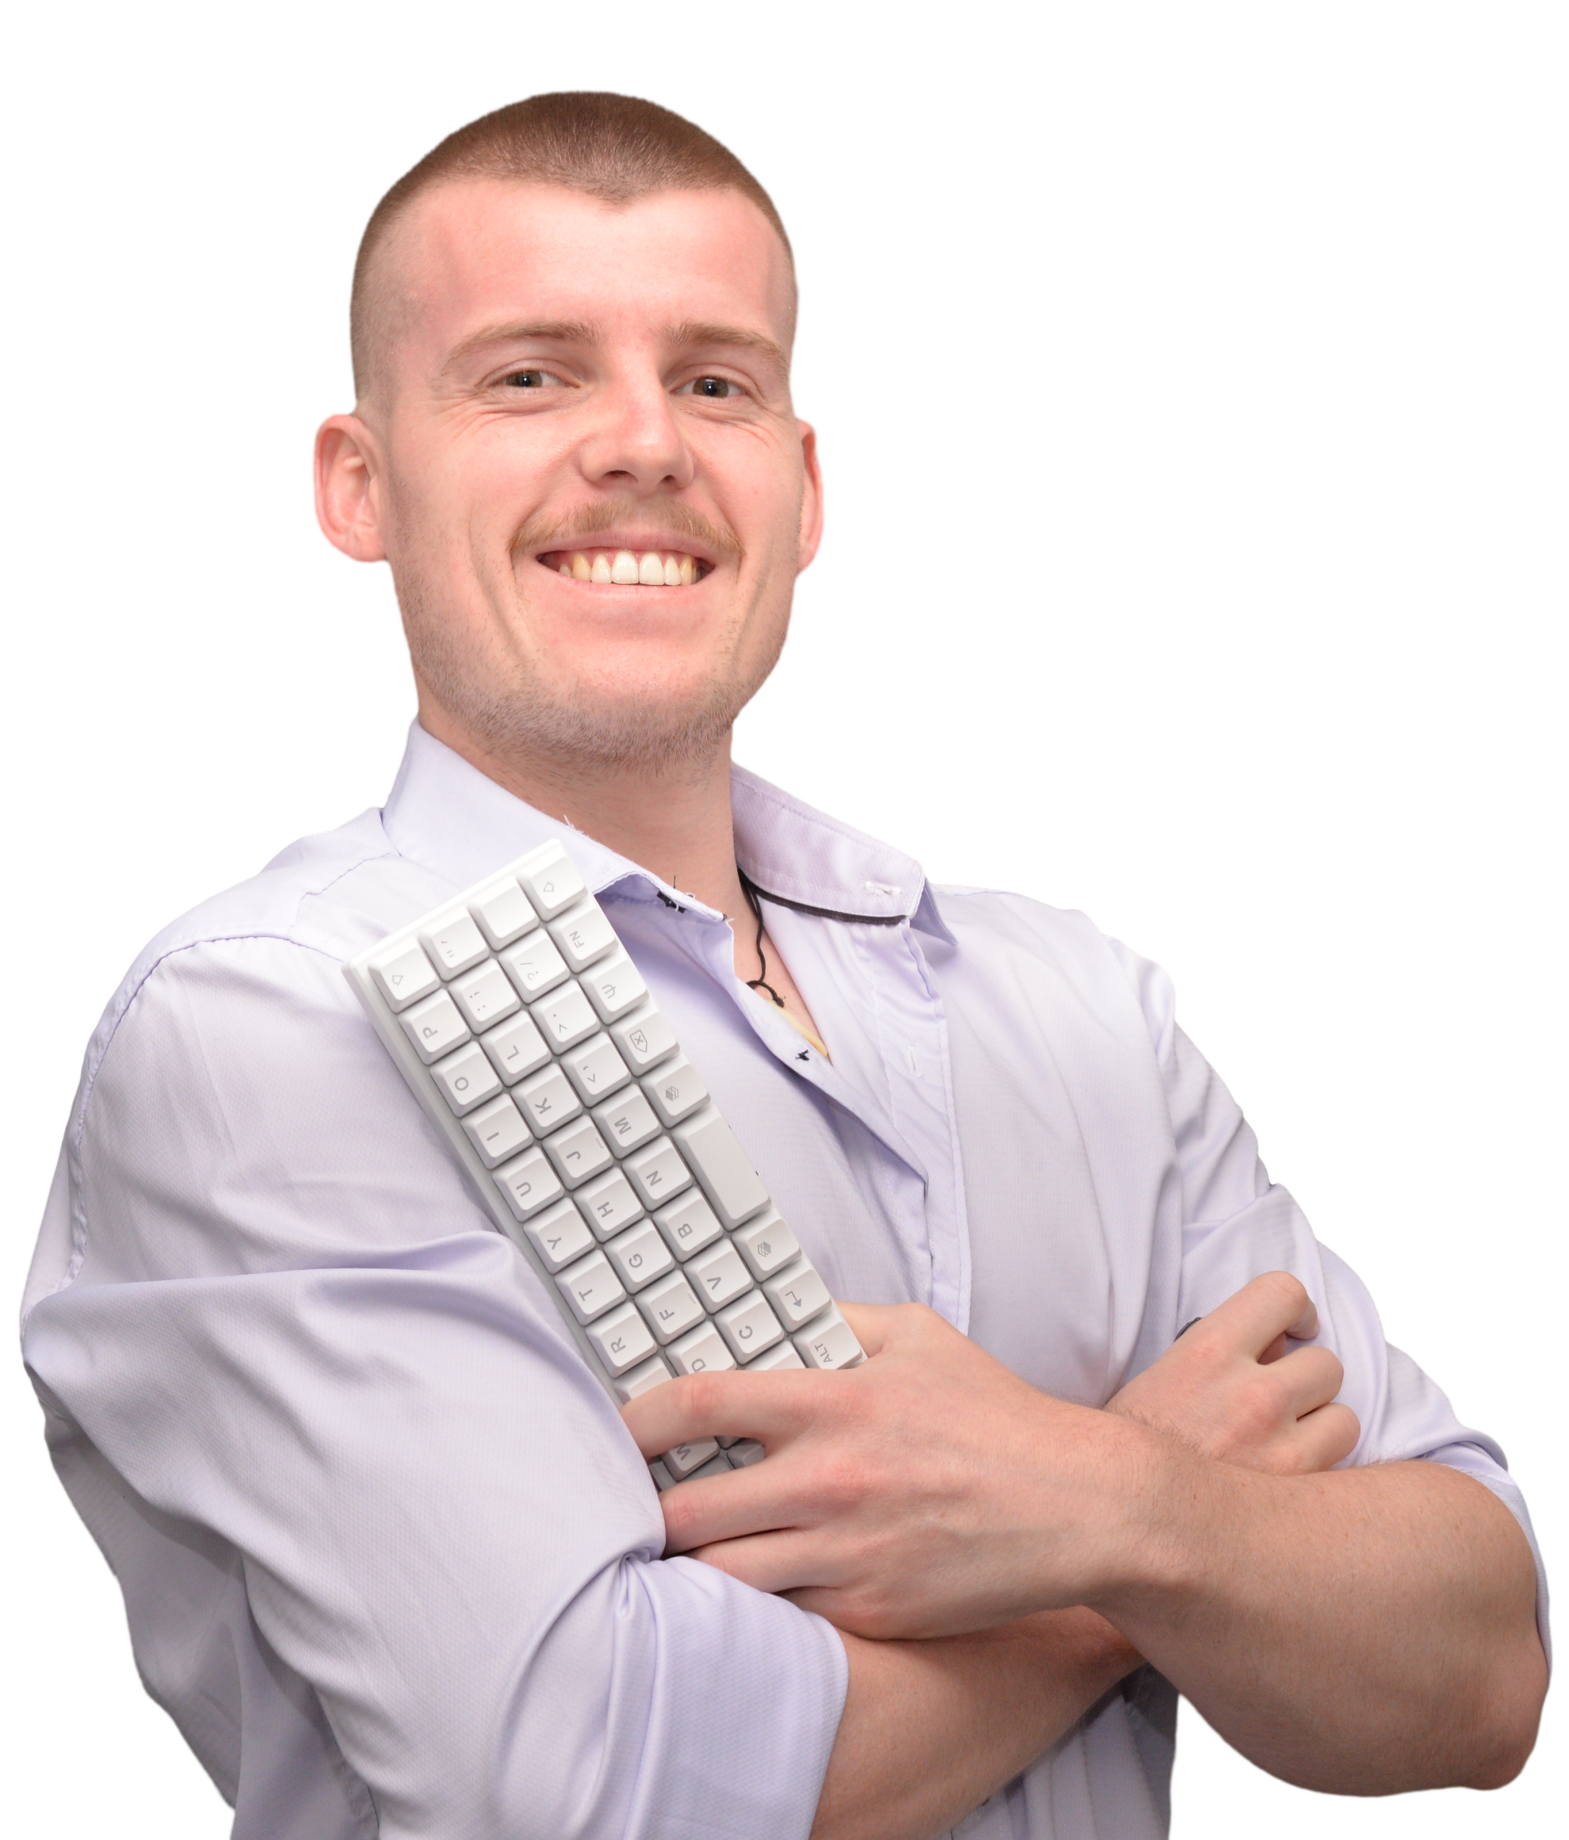
\includegraphics[width=0.9\linewidth]{me-cv}}
	{\footnotesize{Fig 1: Unconventional Profile}}
\end{minipage}

\begin{multicols*}{2}
	\section*{About me}
	\paragraph*{Background:}
	Hailing from what my friends affectionately call a 'singing cult,' my formative years were steeped in music and the performing arts. Now, I've traded sheet music for syntax; my compositions resonate through elegant algorithms, harmonizing data structures and orchestrating efficient solutions.
	\paragraph*{Present:}
	With 3 years of industry experience as a Software Engineer, my technical are currently anchored in \code{TypeScript}, \code{C\#}; complemented by a wide array of technologies. Today, I stand as a bright, bubbly, resilient, and reliable individual.
	\paragraph*{Future:}
	My professional goals center around specializing in backend development, particularly in the realmof network technologies. I'm prepared to bring my distinctive mix of creativity and expertise to exciting projects. Are you ready for me?

	\section*{Work History}
	\subsection*{Z Energy - \texttt{Intermediate Developer}}
	{\footnotesize{May 2022 - Present}}
	\begin{itemize}
		\item \textbf{Programming:}
		      \subitem Proficiency in \code{TypeScript} and \code{C\#} for building applications.
		      \subitem Experience with \code{Azure Cloud} services and infrastructure.
		      \subitem Development of infrastructure as code using \code{Terraform}.
		      \subitem Setup and management of CI/CD pipelines with \code{GitHub Actions} and \code{Azure Pipelines}.
		\item \textbf{Software Development Life Cycle:}
		      \subitem Involvement in the enhancement and modernization of legacy systems.
		      \subitem Understanding of aligning systems with current standards and preparing for future advancements.
		\item \textbf{Incident Investigations:}
		      \subitem Experience with team-based and individual analysis within the Azure Portal.
		      \subitem Ability to identify and resolve discrepancies in code and systems.
	\end{itemize}


\end{multicols*}

\end{document}